%% TeXworks instructions:
% !TeX root = ./report.tex
% !TEX encoding = UTF-8 Unicode
%% !TEX program = arara
%% !TEX TS-program = arara
% !TeX spellcheck = it-IT

% arara: pdflatex: { synctex: yes, action: batchmode, options: "-halt-on-error -file-line-error-style" }
% arara: pdflatex: { synctex: yes, action: nonstopmode, options: "-halt-on-error -file-line-error-style" }

%% Generate a report.xmpdata file with title and authors for PDF/A-compliant format %%
\begin{filecontents*}{\jobname.xmpdata}
    \Title{Maraph1-mp Project Report}
    \Author{Nicholas Brasini\sep Gjulio Jakova\sep Federico Naldini\sep Jacopo Riciputi}
\end{filecontents*}

\documentclass[%
    a4paper,            % specifica il formato A4 (default: letter)
    10pt,               % specifica la dimensione del carattere a 10
    oneside,            % serve per impaginare per stampa solo fronte
    notitlepage         % mette il titolo in una pagina separata (solo per article)
]{article}

\usepackage{a4wide}             % consente di avere più spazio nell'A4

%% ORDINE IMPORTANTE INIZIO %%%%%%%%%%%%
\usepackage[T1]{fontenc}        % serve per impostare la codifica di output del font
\usepackage{textcomp}           % serve per fornire supporto ai Text Companion fonts
\usepackage[utf8]{inputenc}     % serve per impostare la codifica di input del font
\usepackage[
    english,            % utilizza l'inglese come lingua secondaria
    italian             % utilizza l'italiano come lingua primaria
]{babel}                        % serve per scrivere Indice, Capitolo, etc in Italiano

\usepackage{lmodern}            % carica una variante Latin Modern prodotto dal GUST
%% ORDINE IMPORTANTE FINE %%%%%%%%%%%%%%

\usepackage{indentfirst}        % serve per avere l'indentazione nel primo paragrafo
\usepackage{setspace}           % serve a fornire comandi di interlinea standard
\usepackage{xcolor}             % serve per la gestione dei colori nel testo
\usepackage{graphicx}           % serve per includere immagini e grafici

\graphicspath{{./images/}}

\usepackage[%
    strict,             % rende tutti gli warning degli errori
    autostyle,          % imposta lo stile in base al linguaggio specificato in babel
    english=american,   % imposta lo stile per l'inglese
    italian=guillemets  % imposta lo stile per l'italiano
]{csquotes}                     % serve a impostare lo stile delle virgolette

\usepackage{multirow}           % aggiunge la possibilità di raggruppare celle su più righe nelle tabelle

\onehalfspacing%                % Imposta interlinea a 1,5 ed equivale a \linespread{1,5}

\setcounter{secnumdepth}{2}     % Numera fino alla sottosezione nel corpo del testo
\setcounter{tocdepth}{3}        % Numera fino alla sotto-sottosezione nell'indice

\usepackage[%
    depth=3,            % equivale a bookmarksdepth di hyperref
    open=false,         % equivale a bookmarksopen di hyperref
    numbered=true       % equivale a bookmarksnumbered di hyperref
]{bookmark}                     % Gestisce i segnalibri meglio di hyperref
\usepackage{hyperref}           % Gestisce tutte le cose ipertestuali del pdf
\hypersetup{%
    pdfpagemode={UseNone},
    hidelinks,          % nasconde i collegamenti (non vengono quadrettati)
    hypertexnames=false,
    linktoc=all,        % inserisce i link nell'indice
    unicode=true,       % only Latin characters in Acrobat’s bookmarks
    pdftoolbar=false,   % show Acrobat’s toolbar?
    pdfmenubar=false,   % show Acrobat’s menu?
    plainpages=false,
    breaklinks,
    pdfstartview={Fit},
    pdfauthor={Nicholas Brasini, Gjulio Jakova, Federico Naldini, Jacopo Riciputi},
    pdfcreator={Nicholas Brasini, Gjulio Jakova, Federico Naldini, Jacopo Riciputi},
    pdftitle={Maraph1-mp Project Report},
    pdflang={it}
}
%\usepackage[a-1b]{pdfx}
\usepackage[%
    english,italian,    % definizione delle lingue da usare
    nameinlink          % inserisce i link nei riferimenti
]{cleveref}                     % permette di usare riferimenti migliori dei \ref e dei varioref

\title{\LARGE{\textbf{Maraph1-mp Project Report}}}

\author{%
    Nicholas~Brasini\\%
    Gjulio~Jakova\\%
    Federico~Naldini\\%
    Jacopo~Riciputi
}

\date{%
    \small{Paradigmi di Programmazione e Sviluppo}\\%
    \small{Anni accademici 2017--2018 e 2018--2019}
}

\begin{document}

    \maketitle

    \section{Processo di sviluppo}\label{sec:process}
      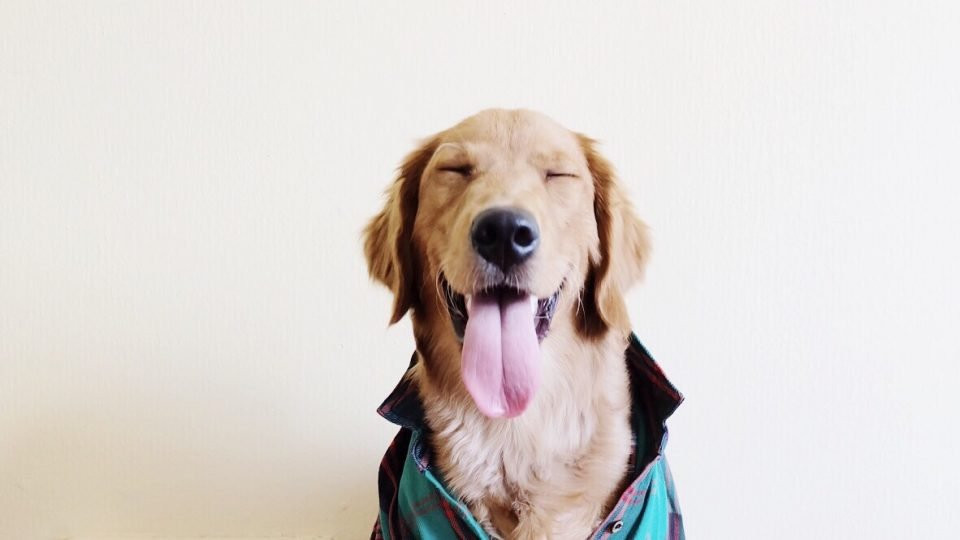
\includegraphics{images/happyDog}
        \subsection{Metodologia di sviluppo}\label{subsec:metodology}
            \subsubsection{Modalità di divisione dei task}\label{subsub:task}
            \subsubsection{Interazioni pianificate}\label{subsub:interations}
            \subsubsection{Modalità di revisione dei task}\label{subsub:revision}
        \subsection{Strumenti adottati}\label{subsec:tools}
            \subsubsection{Linguaggi}\label{subsub:languages}
            \subsubsection{Framework}\label{subsub:framework}
            \subsubsection{Continuous Integration}\label{subsub:ci}
    \section{Requisiti}\label{sec:requirements}
        \subsection{Requisiti utente}\label{subsec:requirements:business}
        \subsection{Requisiti funzionali}\label{subsec:requirements:functional}
            \subsubsection[Gioco]{Regole del gioco}\label{subsub:requirements:game}
            \subsubsection[Autenticazion]{Servizio di autenticazione}\label{subsub:requirements:auth}
            \subsubsection[Stanze di gioco]{Servizio delle stanze di gioco}\label{subsub:requirements:lobby}
            \subsubsection[Service discovery]{Servizio di discovery dei servizi}\label{subsub:requirements:discovery}
            \subsubsection[Interfaccia utente]{Interfaccia grafica per l'utente}\label{subsub:requirements:gui}
        \subsection{Requisiti non funzionali}\label{subsec:requirements:notFunctional}
        \subsection{Requisiti implementativi}\label{subsec:requirements:implementative}
    \section{Design architetturale}\label{sec:design}
        \subsection[Architettura]{Architettura e pattern utilizzati}\label{subsec:architecture}
            \subsubsection{Architettura server-side}\label{subsub:architecture:server}
            \subsubsection{Architettura client-side}\label{subsub:architecture:client}
        \subsection{Tecnologie}\label{subsec:technologies}
    \section{Design di dettaglio}\label{sec:design:details}
    \section{Implementazione}\label{sec:implementation}
        \subsection{Nicholas Brasini}\label{subsec:maltoni}
        \subsection{Gjulio Jakova}\label{subsec:semprini}
        \subsection{Federico Naldini}\label{subsec:soro}
        \subsection{Jacopo Riciputi}\label{subsec:valgimigli}
    \section{Retrospettiva}\label{sec:retrospective}

\end{document}
